\chapter{Tecnología}

\section{Infraestructura}
El punto de vista de Infraestructura contiene los elementos de infraestructura de software y hardware que soportan la capa de aplicación, como dispositivos físicos, redes o software del sistema (por ejemplo, sistemas operativos, bases de datos y middleware). \cite{ArchiMat55:online} \vspace{\baselineskip}

Para el caso de estudio se puede ver como va a estar distribuida la aplicación, las bases de datos a utilizar en el back, como lo son mongoDB y postgres, y basado en un SO Linux, adicionalmente la App que va al celular, se basa en un sistema operativo de Android y en una base de datos de Mysql.

\subsection{Modelo}
\begin{figure}[h!]
	\centering
	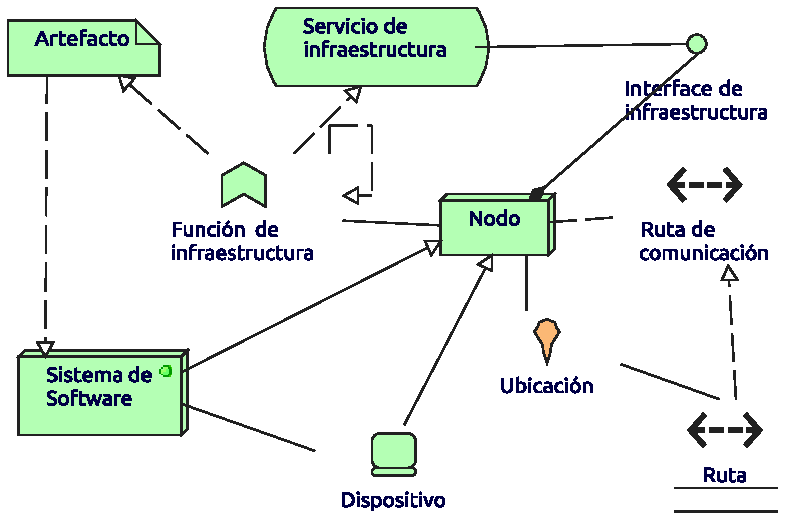
\includegraphics[width=0.8\linewidth]{Arquitectura/Tecnologia/imgs/insfraestructuraMetamodelo.pdf}
	\caption{Modelo: Infraestructura}
\end{figure}
\newpage
\subsection{Caso de Estudio}

\begin{figure}[h!]
	\centering
	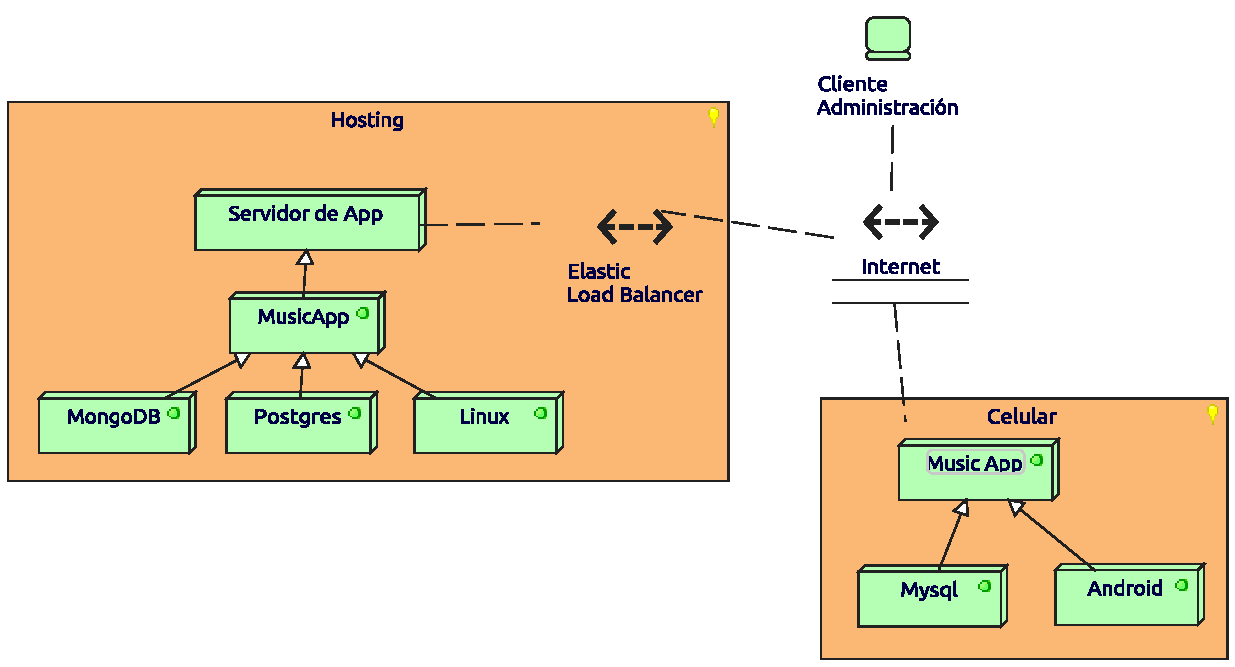
\includegraphics[width=\linewidth]{Arquitectura/Tecnologia/imgs/insfraestructura.pdf}
	\caption{Caso de Estudio: Infraestructura}
\end{figure}

\newpage

\section{Uso de Infraestructura}
El punto de vista Uso de infraestructura muestra cómo las aplicaciones son compatibles con el software y la infraestructura del hardware: los servicios de infraestructura son entregados por los dispositivos; el software del sistema y las redes que se proporcionan a las aplicaciones. \cite{ArchiMat55:online} \vspace{\baselineskip}

Este diagrama enfocado al caso de estudio se puede ver como están organizados los diferentes componentes que integran la app y también podemos ver los sistemas externos que apoyan la funcionalidad de la app como lo son las pasarelas de pago y los sistemas de recomendación.
\subsection{Modelo}
\begin{figure}[h!]
	\centering
	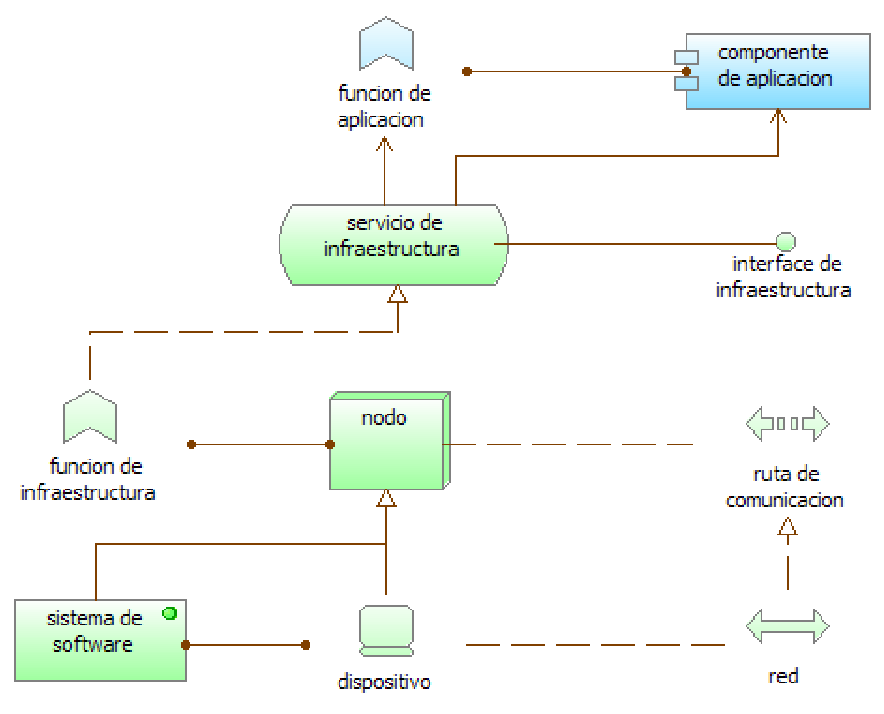
\includegraphics[width=0.8\linewidth]{Arquitectura/Tecnologia/imgs/uso.PNG}
	\caption{Modelo: Uso de Infraestructura}
\end{figure}
\newpage
\subsection{Caso de Estudio}

\begin{figure}[h!]
	\centering
	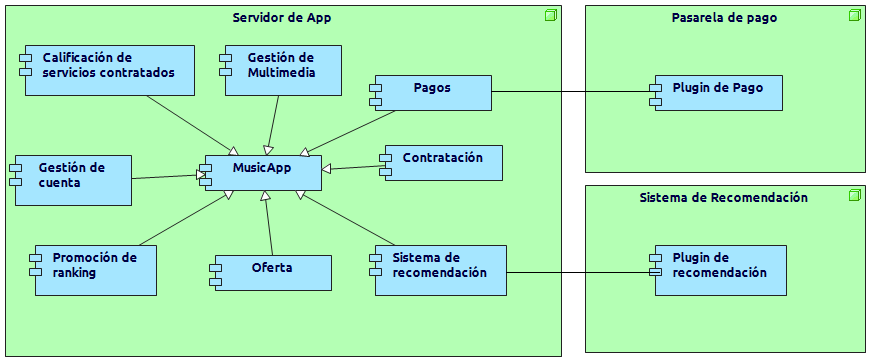
\includegraphics[width=\linewidth]{Arquitectura/Tecnologia/imgs/uso2.png}
	\caption{Caso de Estudio: Uso de Infraestructura}
\end{figure}

\newpage

\section{Estructura de Información}
El punto de vista estructura de información es comparable a los modelos tradicionales de información creados en el desarrollo de casi cualquier sistema de información. Se muestra la estructura de la información utilizada en la empresa o en un proceso de negocio específico o aplicación, en términos de tipos de datos o las estructuras de clase (orientado a objetos). Además, puede mostrar cómo la información a nivel empresarial está representado a nivel de aplicación en la forma de las estructuras de datos utilizadas allí, y cómo éstas son entonces mapeados sobre la infraestructura subyacente; por ejemplo, por medio de un esquema de base de datos. \cite{ArchiMat55:online} \vspace{\baselineskip}

En este modelo para el caso de estudio, se puede ver una parte del modelo de datos, enfocado a la funcionalidad de ver las ofertas de músicos, se puede ver las entidades que se ven involucradas en este proceso, cómo lo es la información de los músicos, la categoría a la que pertenece, las reservaciones que tiene, y las calificaciones o comentarios que ha tenido.

\subsection{Modelo}
\begin{figure}[h!]
	\centering
	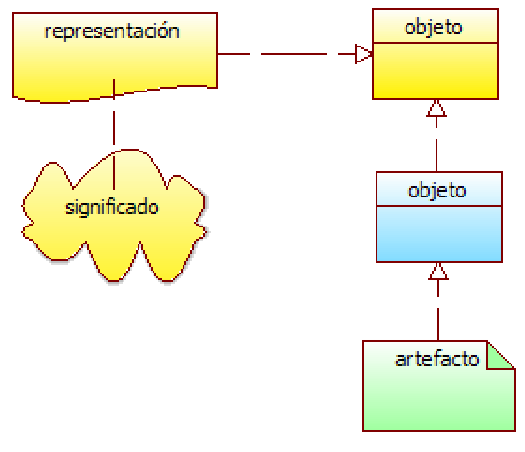
\includegraphics[width=0.8\linewidth]{Arquitectura/Tecnologia/imgs/estructuraMetamodelo.PNG}
	\caption{Modelo: Estructura de Información}
\end{figure}
\newpage
\subsection{Caso de Estudio}

\begin{figure}[h!]
	\centering
	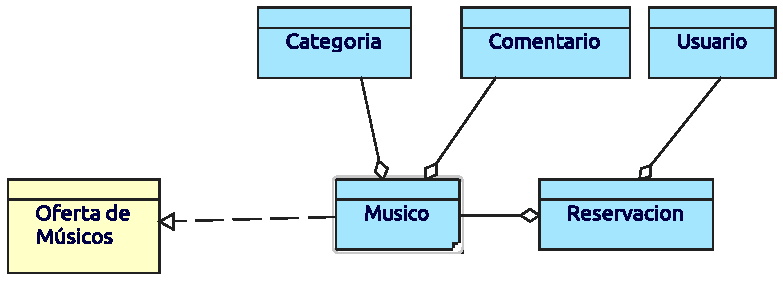
\includegraphics[width=\linewidth]{Arquitectura/Tecnologia/imgs/estructura.pdf}
	\caption{Caso de Estudio: Estructura de Información}
\end{figure}

\newpage

\section{Realización del servicio}
El punto de vista de servicio de Realización se utiliza para mostrar cómo uno o más servicios de negocios son realizados por los procesos subyacentes (y algunas veces por componentes de la aplicación). Por lo tanto, se forma el puente entre el punto de vista de los productos comerciales y la vista de procesos de negocio. Proporciona una "Vista desde el exterior en uno o más procesos de negocio. \cite{ArchiMat55:online} \vspace{\baselineskip}

El punto de vista de servicio de Realización muestra la perspectiva general desde el cliente del proceso de búsqueda y contratación de músicos, el cual es el eje del negocio y los diferentes roles en el proceso.

\subsection{Modelo}
\begin{figure}[h!]
	\centering
	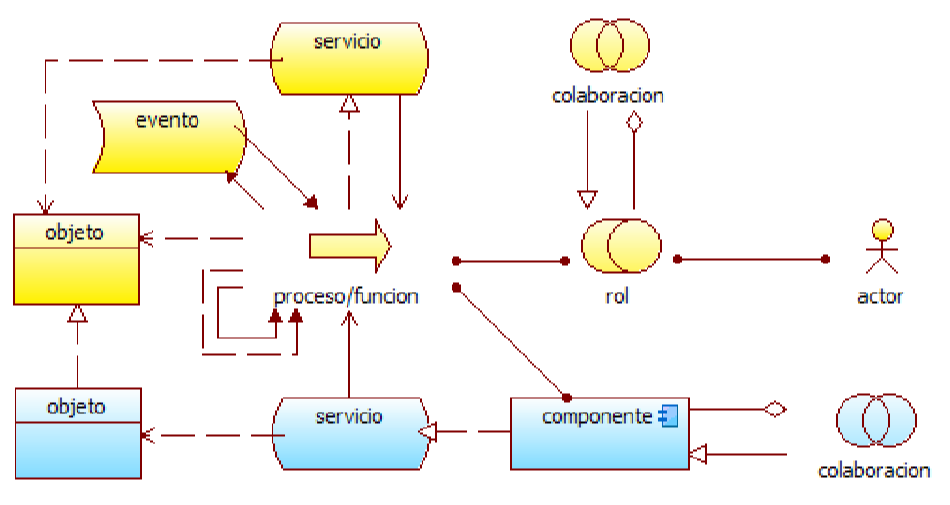
\includegraphics[width=\linewidth]{Arquitectura/Tecnologia/imgs/realizacionMetamodelo.PNG}
	\caption{Modelo: Realización del servicio}
\end{figure}
\newpage
\subsection{Caso de Estudio}

\begin{figure}[hbt!]
	\centering
	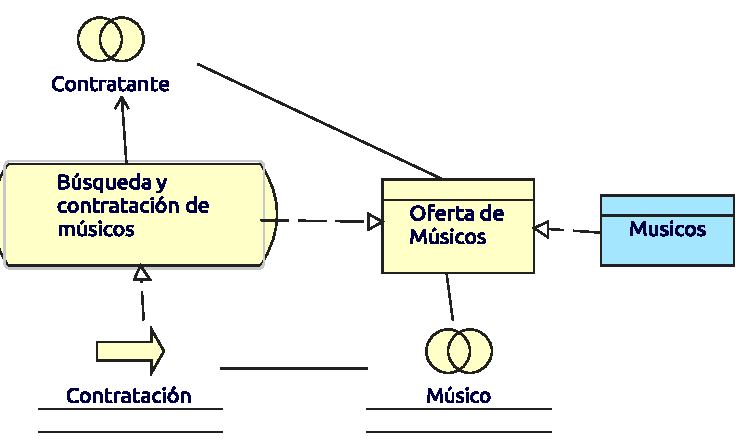
\includegraphics[width=\linewidth]{Arquitectura/Tecnologia/imgs/realizacion.pdf}
	\caption{Caso de Estudio: Realización del servicio}
\end{figure}

\newpage

\section{Capas}
\subsection{Modelo}
En este modelo podemos ver de forma genérica los principales componentes de las diferentes capas de las aplicaciones mostradas hasta el momento. \\

Se pueden ver las capas de Negocio, Aplicación e Infraestructura, y su relación con la principal acción de Negocio.
\subsection{Caso de Estudio}

\begin{figure}[hbt!]
	\centering
	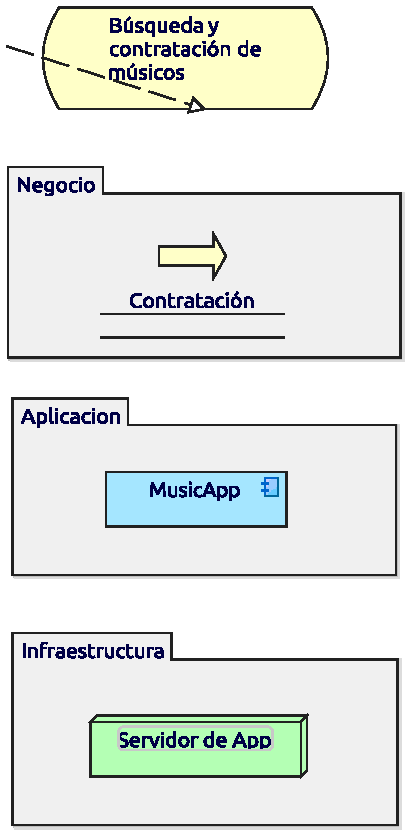
\includegraphics[width=0.4\linewidth]{Arquitectura/Tecnologia/imgs/capas.pdf}
	\caption{Caso de Estudio: Capas}
\end{figure}
